% Sandia National Laboratories is a multimission laboratory managed and
% operated by National Technology & Engineering Solutions of Sandia, LLC, a
% wholly owned subsidiary of Honeywell International Inc., for the U.S.
% Department of Energy’s National Nuclear Security Administration under
% contract DE-NA0003525.

% Copyright 2002-2019 National Technology & Engineering Solutions of Sandia,
% LLC (NTESS).


%% Acknowledgements, Trademarks, and contact information for the Xyce
%% project.
\HeadingC{Acknowledgements}
The authors would like to acknowledge the entire Sandia National
Laboratories electrical modeling community, for their support 
on this project.  This includes, but is not limited to, Bill Ballard,
Dave Shirley, Carolyn Bogdan, Chuck Hembree, 
Biliana Paskeleva, Ken Kambour, Brian Owens, and Nathan Nowlin.

\HeadingC{Trademarks}
The information herein is subject to change without notice.\\[0.5em]
Copyright \copyright{} 2002-2014 Sandia Corporation.  All rights
reserved.\\
\XyceTM{} Electronic Simulator and \XyceTM{} trademarks of Sandia
Corporation.\\
Portions of the \XyceTM{} code are:  \\
Copyright \copyright{} 2002, The Regents of the University of California. \\
Produced at the Lawrence Livermore National Laboratory. \\
Written by Alan Hindmarsh, Allan Taylor, Radu Serban. \\
UCRL-CODE-2002-59 \\
All rights reserved. \\[0.5em]
ModelSim is a registered trademark of Mentor Graphics, Inc.\\[0.5em]
Orcad, Orcad Capture, PSpice and Probe are registered trademarks of Cadence Design Systems, Inc.\\[0.5em]
HSpice is a registered trademarks of Synopsys, Inc.\\[0.5em]
%Silicon Graphics, the Silicon Graphics logo and IRIX are registered trademarks of Silicon Graphics, Inc.\\[0.5em]
Microsoft, Windows and Windows 7 are registered trademark of Microsoft
Corporation.\\[0.5em]
%Solaris and UltraSPARC are registered trademarks of Sun Microsystems Corporation. \\[0.5em]
%Medici, DaVinci and Taurus are registered trademarks of Synopsys Corporation.\\[0.5em]
%HP and Alpha are registered trademarks of Hewlett-Packard company.  \\[0.5em]
%Amtec and TecPlot are trademarks of Amtec Engineering, Inc. \\[0.5em]
\Xyce{}'s expression library is based on that inside Spice 3F5 developed by
the EECS Department at the University of California. \\[0.5em]
The EKV3 MOSFET model was developed by the EKV Team of the Electronics Laboratory-TUC of the Technical University of Crete. \\[0.5em]
All other trademarks are property of their respective owners.
\HeadingC{Contacts} \label{Contacts}
Bug Reports \hfill \texttt{\color{XyceDeepRed}http://charleston.sandia.gov/bugzilla} \\
Email \hfill \texttt{\color{XyceDeepRed}xyce-support@sandia.gov} \\
World Wide Web \hfill \texttt{\color{XyceDeepRed}http://xyce.sandia.gov/}

\vspace*{\fill}
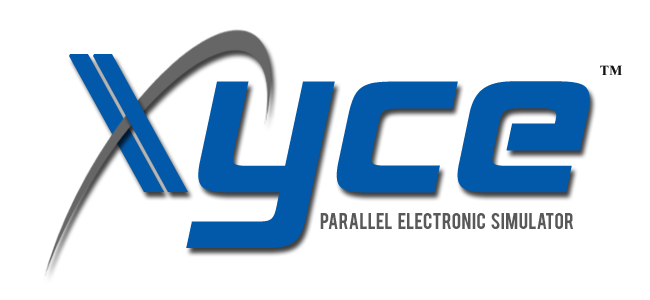
\includegraphics[height=0.5in]{../Common_Guide_Files/xyce_flat_white}
\hfill
\includegraphics[height=0.5in]{../Common_Guide_Files/snllineblubrd}

